\section{Keeping Up With the M\"{o}biuseseses}
% riemann sphere and fractional linear transformations
M\"{o}bius transformations, or fractional linear transformations (FLTs), are worth studying as a sidenote here they are interesting conformal mappings of regions. These were discussed in HCSSiM's PJ 5, but I'll reiterate some of the main points here.

FLTs are functions of the form $f(z) = \frac{az+b}{cz+d}$, where $ad - bc \neq 0$ as to not make the function constant. They are compositions of translations ($f(z) : z \rightarrow z + c, c \in \CC$), rotations/dilations ($f(z) : z \rightarrow rz, r \in \CC$) and a reciprocation $\left(f(z) : z \rightarrow \frac{1}{z}\right)$. Because of this, they can established to be conformal by how they are constructed, geometrically (regular geometric inversion preserves angles, but not orientation... see if you can work this one out!).

In particular, FLTs are nice because they send circles and lines to circles and lines. This is true by construction for translations, rotations, and dilations, but reciprocations require breaking the function down into its real and imaginary parts and computing this explicitly.

Currently, the point $z = - \frac{d}{c}$ is a pole, unless we work in the \textit{one-point compactification of the complex plane}, which is just fancy math speak for ``adding $\infty$ to $\CC$ to complete the plane.'' This also allows us to have $\frac{a}{c}$ in our range, if we're allowed to plug in the point at infinity into our FLTs.

FLTs are fixed by three points -- we can always construct transformations that send the numbers $z_1$, $z_2$, and $z_3$ to $0, \infty$, and 1, respectively, like so:
\[
  f(z) = \frac{z_3-z_2}{z_3-z_1} \cdot \frac{z-z_1}{z-z_2}
\]
That means if we want to generally send $z_1 \rightarrow w_1$, $z_2 \rightarrow w_2$, and $z_3 \rightarrow w_3$, we can construct $f(z)$ such that $z_1 \rightarrow 0$, $z_2 \rightarrow \infty$, and $z_3 \rightarrow 1$, as well constructing $g(z)$ such that $w_1 \rightarrow 0$, $w_2 \rightarrow \infty$, and $w_3 \rightarrow 1$. Then, we can take $h(z) = g^{-1}(f(z))$ to get the unique transformation we want, which shows that transformations are fixed by three points.

With all of that summary out of the way, I'm most interested in talking about looking at the domain/range graphs when it comes to the FLTs. In all of the following examples, I'll provide the domain, and its output range. Note that all of these are conformal -- they preserve orientation and angles, even if they don't look like it! A good way to check orientation -- if you walk around the boundary counterclockwise (including through infinity), the interior should be to the left.

Okay, here are the pictures, and all of them are pretty wacky.  I tried to make Mathematica as unhappy as possible by using the reciprocation as much as possible, so these will look weird:
\begin{center}
  1. $f(z) = \frac{z-1}{z}$ on unit disk $|z| \leq 1$: \\
  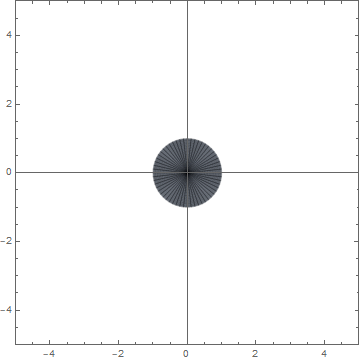
\includegraphics[scale=0.3]{images/mobius1dom.png}
  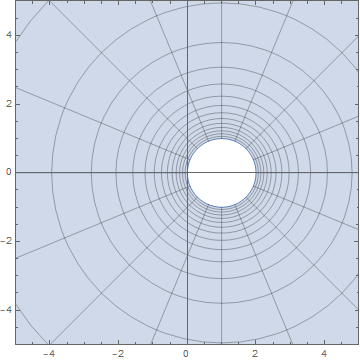
\includegraphics[scale=0.3]{images/mobius1ran.png}
\end{center}
\begin{center}
  2. $f(z) = \frac{z+1}{-z+1}$ on unit disk $|z| \leq 1$: \\
  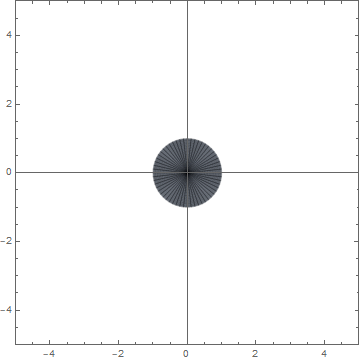
\includegraphics[scale=0.3]{images/mobius1dom.png}
  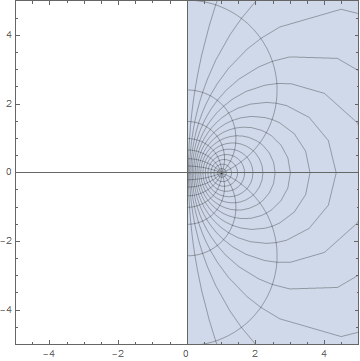
\includegraphics[scale=0.3]{images/mobius2ran.png}
\end{center}
\begin{center}
  3. $f(z) = \frac{1}{z}$ on square -- $\Re(z) \in [-1,1], \Im(z) \in [-1,1]$: \\
  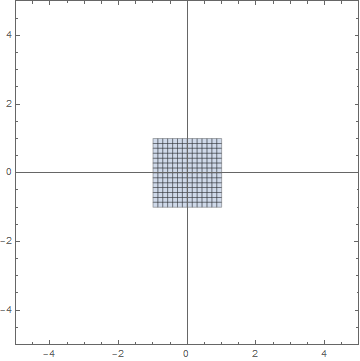
\includegraphics[scale=0.3]{images/mobius3dom.png}
  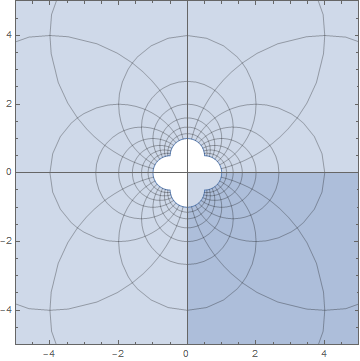
\includegraphics[scale=0.3]{images/mobius3ran.png}
\end{center}
\begin{center}
  4. $f(z) = (1+i)\frac{z-1}{z-i}$ on square -- $\Re(z) \in [0,1], \Im(z) \in [0,4]$: \\
  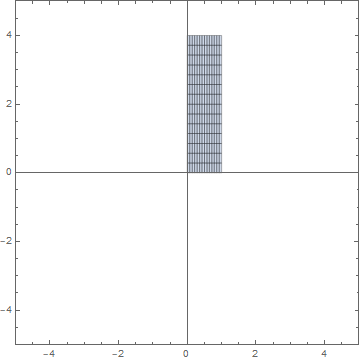
\includegraphics[scale=0.3]{images/mobius4dom.png}
  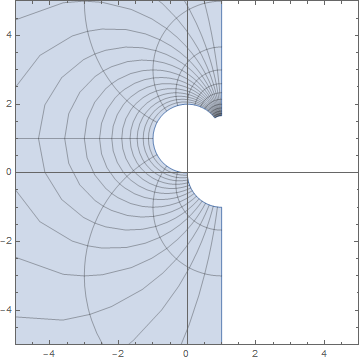
\includegraphics[scale=0.3]{images/mobius4ran.png}
\end{center}
The third example is an example of where Mathematica tries to connect the different infinities encountered near zero, and it ends up overlapping one of the quadrants. I'm not sure how to fix this, because the region is really only supposed to be the plane, minus the cloverleaf in the middle. Work it out for yourself to verify this! Try mapping each of these (directed) segments seperately, remembering to keep the interior to the left. :)